
\chapter{多体Green函数}

在本附录中，我们想给予一个关于多体Green函数（GF）理论的简要概述。这些技术通常不太适用于核理论，然而它们在许多其他多体领域的工作中得到了广泛的应用。Green函数方法的优点是它在构造近似地多体方法时非常灵活，而且Green函数具有直接的物理解释。为了本大纲的简洁性，读者最好自己查阅现有的文献和教科书来了解标准的形式理论\cite{Mi67,AGD65,No64a,Ma67b,FW71}，因此，只有我们的表示方式和一般的不同时，我们才会讨论具体细节。

\section{单粒子Green函数和Dyson方程}

我们想要建立单粒子Green函数的Dyson方程，这里单粒子Green函数定义为
\begin{comment}
为了与现代文献中的符号接轨，这里使用了更现代的写法。
\end{comment}
：
\begin{align*}
G_{\alpha\beta}(t,t^{\prime}) & =(-\mathrm{i})\langle0|\mathcal{T}c_{\alpha}(t)c^{\dagger}_{\beta}(t^{\prime})|0\rangle\\
 & =-\mathrm{i}\theta(t-t^{\prime})\langle0|c_{\alpha}(t)c^{\dagger}_{\beta}(t^{\prime})|0\rangle+\mathrm{i}\theta(t^{\prime}-t)\langle0|c^{\dagger}_{\beta}(t^{\prime})c_{\alpha}(t)|0\rangle
\end{align*}

\begin{comment}
这里是针对费米子定义的。
\end{comment}
这里我们使用下面的一套符号体系：我们用希腊字母$\alpha,\beta$等表示标记一个单粒子态所需的所有量子数，例如动量、自旋、同位旋。重复的指标应当被求和掉或者积掉，除非特别说明。$|\rangle$是$A$粒子体系的真空态，$\mathcal{T}$是编时算符。单粒子算符
\begin{comment}
Heisenberg绘景下的。
\end{comment}
为：
\[
c^{\dagger}_{\alpha}(t)=\mathrm{e}^{\mathrm{i}Ht/\hbar}c^{\dagger}_{\alpha}\mathrm{e}^{-\mathrm{i}Ht/\hbar}
\]

其随时间的演化由两体Hamilton量决定
\begin{comment}
这里采用了单体部分对角的表象，并不影响下面一些普遍结论的证明。但一般来讲，单体部分不一定对角。
\end{comment}
：
\[
H=\sum_{\alpha}\varepsilon_{\alpha}c^{\dagger}_{\alpha}c_{\alpha}+\frac{1}{4}\sum_{\alpha\beta\gamma\delta}\bar{v}_{\alpha\beta\gamma\delta}c^{\dagger}_{\alpha}c^{\dagger}_{\beta}c_{\delta}c_{\gamma};\quad\varepsilon_{\alpha}=\frac{p^{2}_{\alpha}}{2m}
\]

单粒子Green函数之所以有用，是因为它实际蕴含了许多可观测量，例如：
\begin{enumerate}
\item 单粒子密度矩阵
\begin{comment}
这意味着任意单体算符的期待值可以由此求出。
\end{comment}
：
\[
\rho_{\alpha\beta}=\langle0|c^{\dagger}_{\beta}c_{\alpha}|0\rangle=-\mathrm{i}\lim_{t^{\prime}-t\rightarrow0^{+}}G_{\alpha\beta}(t,t^{\prime})=\frac{1}{2\mathrm{\pi}\mathrm{i}}\int\mathrm{d}\omega\,G_{\alpha\beta}(\omega)
\]

这里$G_{\alpha\beta}(\omega)$是$G_{\alpha\beta}(t,t^{\prime})$的Fourier变换：
\[
G_{\alpha\beta}(\omega)=\int\mathrm{d}(t-t^{\prime})\mathrm{e}^{\mathrm{i}\omega(t-t^{\prime})}G_{\alpha}(t,t^{\prime})
\]

\item $A\pm1$粒子系统的激发能：这可以通过插入完备基看出：
\begin{align*}
G_{\alpha\beta}(t,t^{\prime}) & =-\mathrm{i}\sum_{n}\theta(t-t^{\prime})\langle0|c_{\alpha}|n,A+1\rangle\langle n,A+1|c^{\dagger}_{\beta}|0\rangle\mathrm{e}^{-(\mathrm{i}/\hbar)(E^{A+1}_{n}-E^{A}_{0})(t-t^{\prime})}\\
 & +\mathrm{i}\sum_{n}\theta(t^{\prime}-t)\langle0|c^{\dagger}_{\beta}|n,A-1\rangle\langle n,A-1|c_{\alpha}|0\rangle\mathrm{e}^{-(\mathrm{i}/\hbar)(E^{A}_{0}-E^{A-1}_{n})(t-t^{\prime})}
\end{align*}

或者写成
\begin{comment}
这被称为Lehmann谱表示。
\end{comment}
：
\[
G_{\alpha\beta}(\omega)=\hbar\sum_{n}\frac{\langle0|c_{\alpha}|n,A+1\rangle\langle n,A+1|c^{\dagger}_{\beta}|0\rangle}{\hbar\omega-(E^{A+1}_{n}-E^{A}_{0})+\mathrm{i}\eta}+\hbar\sum_{n}\frac{\langle0|c^{\dagger}_{\beta}|n,A-1\rangle\langle n,A-1|c_{\alpha}|0\rangle}{\hbar\omega-(E^{A}_{0}-E^{A-1}_{n})-\mathrm{i}\eta}
\]

这里$|n\rangle$是Hamilton量的精确本征矢：
\[
H|n,A\pm1\rangle=E^{A\pm1}_{n}|n,A\pm1\rangle
\]

\item 基态能量：
\begin{align}
E_{0} & =\langle0|H|0\rangle=-\frac{\mathrm{i}}{2}\lim_{t^{\prime}\rightarrow t^{+}}\sum_{\alpha}(\varepsilon_{\alpha}+\mathrm{i}\hbar\frac{\partial}{\partial t})G_{\alpha\alpha}(t,t^{\prime})\nonumber \\
 & =\frac{1}{2}\int\frac{\mathrm{d}\omega}{2\mathrm{\pi}\mathrm{i}}\,\sum_{\alpha}(\varepsilon_{\alpha}+\hbar\omega)G_{\alpha\alpha}(\omega)\label{eq:F_7}
\end{align}

这里我们已经利用了算符$c$和$c^{\dagger}$的运动方程：
\begin{align}
\mathrm{i}\hbar\frac{\partial}{\partial t}c_{\alpha}(t) & =\varepsilon_{\alpha}c_{\alpha}(t)+j(t)\label{eq:EOM of a}\\
-\mathrm{i}\hbar\frac{\partial}{\partial t}c^{\dagger}_{\alpha}(t) & =\varepsilon_{\alpha}c^{\dagger}_{\alpha}(t)+j^{\dagger}(t)\nonumber 
\end{align}

这里：
\[
j(t)=\frac{1}{2}\bar{v}_{\alpha\beta\gamma\delta}c^{\dagger}_{\beta}(t)c_{\delta}(t)c_{\gamma}(t)
\]

\begin{booknote*}
运动方程即通过Heisenberg运动方程得出：
\begin{align*}
\mathrm{i}\hbar\frac{\partial}{\partial t}c_{\alpha}(t) & =[c_{\alpha}(t),H]=\mathrm{e}^{\mathrm{i}Ht/\hbar}[c_{\alpha},H]\mathrm{e}^{-\mathrm{i}Ht/\hbar}
\end{align*}

计算即可得到上述运动方程。由此：
\[
\sum_{\alpha}\left(\mathrm{i}\hbar\frac{\partial}{\partial t}-\varepsilon_{\alpha}\right)\langle0|c^{\dagger}_{\alpha}(t^{\prime})c_{\alpha}(t)|0\rangle=\frac{1}{2}\sum_{\alpha\beta\gamma\delta}\bar{v}_{\alpha\beta\gamma\delta}\langle0|c^{\dagger}_{\alpha}(t^{\prime})c^{\dagger}_{\beta}(t)c_{\delta}(t)c_{\gamma}(t)|0\rangle
\]

可以发现，左侧实际上为：
\[
-\mathrm{i}\sum_{\alpha}\lim_{t^{\prime}\rightarrow t^{+}}\left(\mathrm{i}\hbar\frac{\partial}{\partial t}-\varepsilon_{\alpha}\right)G_{\alpha\alpha}(t,t^{\prime})
\]

我们又有：
\[
\sum_{\alpha}\varepsilon_{\alpha}\langle0|c^{\dagger}_{\alpha}c_{\alpha}|0\rangle=-\mathrm{i}\sum_{\alpha}\varepsilon_{\alpha}\lim_{t^{\prime}\rightarrow t^{+}}G_{\alpha\alpha}(t,t^{\prime})
\]

进而很容易得到：

\begin{align*}
E_{0} & =\langle0|H|0\rangle=-\mathrm{i}\sum_{\alpha}\varepsilon_{\alpha}\lim_{t^{\prime}\rightarrow t^{+}}G_{\alpha\alpha}(t,t^{\prime})-\frac{\mathrm{i}}{2}\sum_{\alpha}\lim_{t^{\prime}\rightarrow t^{+}}\left(\mathrm{i}\hbar\frac{\partial}{\partial t}-\varepsilon_{\alpha}\right)G_{\alpha\alpha}(t,t^{\prime})\\
 & =-\frac{\mathrm{i}}{2}\sum_{\alpha}\lim_{t^{\prime}\rightarrow t^{+}}\left(\mathrm{i}\hbar\frac{\partial}{\partial t}+\varepsilon_{\alpha}\right)G_{\alpha\alpha}(t,t^{\prime})
\end{align*}
\end{booknote*}
\end{enumerate}
现在我们继续推导出Dyson方程。利用式 (F.8) 的运动方程，我们可以建立Green函数的运动方程：

\begin{equation}
G^{00-1}(1,2)G(2,1')=\delta(1,1')+G(j(1),1')\label{eq:F_10}
\end{equation}

其中
\begin{equation}
\delta(1,1')=\delta_{11'}\delta(t_{1}-t_{1'})\hbar,\label{eq:F_11}
\end{equation}
且
\[
G^{00-1}(1,1')\equiv[G^{00-1}]_{11'}(t_{1},t_{1'})=\delta(1,1')\left(\mathrm{i}\hbar\frac{\partial}{\partial t_{1'}}-\varepsilon_{1'}\right),
\]
以及
\begin{equation}
G(j(1),1')=-\mathrm{i}\langle0|\mathcal{T}\{j(1)a^{\dagger}(1')\}|0\rangle.\label{eq:F_12}
\end{equation}
再次应用运动方程，我们得到
\begin{equation}
G(j(1),2)G^{00-1}(2,1')=\bar{v}_{1234}\langle0|a^{\dagger}_{2}a_{4}|0\rangle\hbar\delta(t_{1}-t_{1'})+G(j(1),j(1')),\label{eq:F_13}
\end{equation}
其中我们利用了与式 \ref{eq:F_11} 等价的形式：
\begin{equation}
G^{00-1}(1,1')=\left(-\mathrm{i}\hbar\frac{\overleftarrow{\partial}}{\partial t_{1}}-\varepsilon_{1}\right)\delta(1,1')\label{eq:F_14}
\end{equation}
而 $G(j(1),j(1'))$ 由下式给出：
\begin{equation}
G(j(1),j(1'))=-\mathrm{i}\langle0|\mathcal{T}\{j(1)j^{\dagger}(1')\}|0\rangle.\label{eq:F_15}
\end{equation}

Green函数 $G(1,1')$ 的逆算符定义为
\begin{equation}
G^{-1}(1,2)\cdot G(2,1')=\delta(1,1')\label{eq:F_16}
\end{equation}
因此我们可以写出
\begin{equation}
G^{00-1}(1,2)G(2,1')=G^{-1}(1,2)\cdot G(2,3)G^{00-1}(3,4)G(4,1'),\label{eq:F_17}
\end{equation}
结合式 \ref{eq:F_10} 的伴随方程
\begin{equation}
G(1,2)G^{00-1}(2,1')=\delta(1,1')+G(1,j(1')),\label{eq:F_18}
\end{equation}
即可导出关系式
\begin{equation}
G^{00-1}(1,2)G(2,1')=\delta(1,1')+G^{-1}(1,2)G(2,j(3))G(3,1').\label{eq:F_19a}
\end{equation}
按同样的方式，我们还可以导出
\begin{equation}
G(1,2)G^{00-1}(2,1')=\delta(1,1')+G(1,2)G(j(2),3)G^{-1}(3,1').\label{eq:F_19b}
\end{equation}

将式 \ref{eq:F_13} 从右侧乘以单粒子Green函数并利用式 \ref{eq:F_19a}，我们得到：
\begin{equation}
G(j(1),1')=\bar{v}_{1234}\langle0|a^{\dagger}_{2}a_{4}|0\rangle G_{31'}(t_{1},t_{1'})+R(j(1),j(2))G(2,1')\label{eq:F_20}
\end{equation}
其中 \cite{ES69}：
\begin{equation}
R(j(1),j(1'))=G(j(1),j(1'))-G(j(1),2)G^{-1}(2,2')G(2',j(1')).\label{eq:F_21}
\end{equation}
将结果 \ref{eq:F_20} 代入式 \ref{eq:F_10} 中，经过Fourier变换后可得：
\begin{equation}
(\hbar\omega-\varepsilon_{1})G_{11'}(\omega)=\delta_{11'}+M_{12}(\omega)G_{21'}(\omega)\label{eq:F_22a}
\end{equation}
或写为
\begin{equation}
G(1,1')=G^{00}(1,1')+G^{00}(1,2)M(2,2')G(2',1')\label{eq:F_22b}
\end{equation}
其中
\begin{equation}
M_{11'}(\omega)=M^{0}_{11'}+M'_{11'}(\omega),\label{eq:F_23}
\end{equation}
\begin{equation}
M^{0}_{11'}=\bar{v}_{121'4}\rho_{42},\label{eq:F_24}
\end{equation}
\begin{equation}
M'_{11'}(\omega)=R_{j(1)j(1')}(\omega).\label{eq:F_25}
\end{equation}

方程 \ref{eq:F_22a} 即为著名的Dyson方程，而 $M(1,1')$ 是相应的所谓质量算符（mass operator），它包含一个静态（与频率无关）部分
$M^{0}$ 和一个动态（依赖于频率）部分 $M'$。后者的表述形式有些非同寻常，我们稍后将讨论其物理意义。

对 $M(1,1')$ 所作的近似将决定 $G(1,1')$ 的近似。让我们首先采用最简单的近似，完全略去 $M'$；这给出：
\begin{equation}
(\hbar\omega-\varepsilon_{1})g_{11'}(\omega)=\delta_{11'}+\Gamma_{12}g_{21'}(\omega),\label{eq:F_26}
\end{equation}
\begin{equation}
\Gamma_{11'}=\bar{v}_{121'4}\oint\frac{\mathrm{d}\omega}{2\pi\mathrm{i}}g_{42}(\omega).\label{eq:F_27}
\end{equation}
这构成了一组自洽的非线性闭合方程组，等价于第5章的Hartree-Fock方程。将式 \ref{eq:F_26} 中的 $\omega\cdot g_{11'}$
代入式 \ref{eq:F_7}，并注意到由此得出的基态能量表达式恰好具有Hartree-Fock形式 (5.40)，即可最容易地看出这种等价性。同样，当趋向于式
\ref{eq:F_26} 中 $g_{11'}$ 的某一极点时，我们严格重现了Hartree-Fock方程 (5.44)。类比于式
(F.6a, b)，式 \ref{eq:F_26} 的形式解由下式给出：
\begin{equation}
g_{11'}(\omega)=\hbar\left(\frac{1-\rho}{\hbar\omega-h+\mathrm{i}\eta}\right)_{11'}+\hbar\left(\frac{\rho}{\hbar\omega-h-\mathrm{i}\eta}\right)_{11'},\label{eq:F_28}
\end{equation}
其中 $\rho$ 是HF密度算符，而 $h$ 是HF Hamilton量 (5.37)。类似地，在时间坐标空间中我们有：
\begin{equation}
g(1,1')=-\mathrm{i}\left(\Theta(t_{1}-t_{1'})(1-\rho)-\Theta(t_{1'}-t_{1})\rho\right)_{12}\left(\mathrm{e}^{-(\mathrm{i}/\hbar)h(t_{1}-t_{1'})}\right)_{21'}.\label{eq:F_29}
\end{equation}

为了更好地理解质量算符动态部分 \ref{eq:F_25} 的物理意义，我们首先证明：完整的质量算符对应于弹性核子-核散射的最一般能量依赖的光学模型势（optical
model potential）。为证明这一点，我们在动量表象中工作，并按通常的方式 \cite{ES69} 将弹性散射 $S$
矩阵写为：
\begin{equation}
S_{p_{1}p_{1'}}={}^{-}\langle p_{1}|p_{1'}\rangle^{+}\label{eq:F_30}
\end{equation}
其中
\begin{align}
|p\rangle^{\pm} & =\lim_{t\rightarrow\mp\infty}\mathrm{e}^{-\mathrm{i}(p^{2}/2m)t/\hbar}a^{\dagger}_{p}(t)|0\rangle\nonumber \\
 & =\lim_{t\rightarrow\mp\infty}\mathrm{e}^{-\mathrm{i}(E_{p}-H)t/\hbar}a^{\dagger}_{p}|0\rangle;\label{eq:F_31}
\end{align}
\[
E_{p}=\frac{p^{2}}{2m}+E^{A}_{0}.
\]
因此我们可以用式 (F.1) 的单粒子Green函数来表示 $S$ 矩阵：
\begin{equation}
S_{p_{1}p_{1'}}=\mathrm{i}\lim_{\substack{t\rightarrow+\infty\\
t'\rightarrow-\infty
}
}\mathrm{e}^{\mathrm{i}(p^{2}_{1}/2m)t/\hbar}G_{p_{1}p_{1'}}(t-t')\mathrm{e}^{-\mathrm{i}(p^{2}_{1'}/2m)t'/\hbar}.\label{eq:F_32}
\end{equation}

现在我们将方程 \ref{eq:F_22b} 改写为如下形式：
\begin{align}
G(1,1') & =G^{00}(1,1')+G^{00}(1,2)T(2,2')G^{00}(2',1'),\nonumber \\
T(1,1') & =M(1,1')+M(1,2)G^{00}(2,2')T(2',1'),\label{eq:F_33}
\end{align}
其中 $G^{00}$ 是式 \ref{eq:F_11} 的逆算符，即：
\begin{align}
G^{00}_{p_{1}p_{1'}}(t_{1}-t_{1'}) & =-\mathrm{i}\delta_{p_{1}p_{1'}}\exp\left[-\frac{\mathrm{i}}{\hbar}\frac{p^{2}_{1}}{2m}(t_{1}-t_{1'})\right]\nonumber \\
 & \quad\cdot\left(\Theta(t_{1}-t_{1'})\cdot\Theta(p^{2}_{1}/2m-\lambda)-\Theta(t_{1'}-t_{1})\cdot\Theta(\lambda-p^{2}_{1}/2m)\right),\label{eq:F_34}
\end{align}
其中 $\lambda$ 是Fermi能，即 $G^{00}$ 是完全自由的多体系统的单粒子Green函数。式 \ref{eq:F_33}
与式 \ref{eq:F_22b} 的等价性可通过简单迭代确立。利用式 \ref{eq:F_34} 和式 \ref{eq:F_33}
执行时间极限，我们求得式 \ref{eq:F_32}：
\begin{equation}
S_{p_{1}p_{1'}}=\delta_{p_{1}p_{1'}}-2\pi\mathrm{i}T_{p_{1}p_{1'}}(\omega=p^{2}_{1}/2m)\delta\left((p^{2}_{1}-p^{2}_{1'})/2m\right).\label{eq:F_35}
\end{equation}

因此我们看到，由式 \ref{eq:F_33} 定义的矩阵 $T(1,1')$ 对应于弹性核子-核散射的散射 $T$ 矩阵。式
\ref{eq:F_33} 中的第二个方程随后还告诉我们，$M(1,1')$ 对应于光学模型势，后者通常自然是能量依赖且非局域的。一般而言，光学势是借助Feshbach投影算符形式（参见4.3.2节），利用壳模型态的完备集
$1p,2p-1h,3p-2h,\dots$ 并投影掉 $2p-1h,3p-2h,\dots$ 分量而导出的。因此，我们看到质量算符的物理涵义是一个“有效”单粒子势，其中在动态部分内隐藏了与所有更高阶组态的耦合\footnote{通过Feshbach投影算符形式定义的光学势与此处在微扰论处理中所给出的光学势之间的等价性是一个相当精细的问题，我们在此不作展开。}。正如对所有有效势一样，我们也可以“展开”质量算符的能量依赖性，转而在更大的空间中写出一个矩阵方程（稍后将给出示例）。质量算符通常是一个复且非Hermite的量，照例在计算此类算符的本征矢和本征值时必须遵循专门的规则。我们不拟深入探讨这些细节，读者可参阅文献
\cite[附录C]{BD71}。

正如我们所见，单粒子Green函数的计算依赖于对质量算符的了解。为了能够获得关于它的某种近似，我们首先必须学习如何为 $M$ 构建微扰级数。

\section{微扰论}

在深入讨论微扰论的细节之前，我们先简要介绍如何用图形表示我们将要借助Green函数理论推导出的各种表达式。这些图形表示对于一目了然地把握一个最终可能相当复杂的方程的物理内容非常有用。然而我们希望强调的是，我们将尽可能避免完全依靠纯图形论据来推导关系式；相反，我们将努力解析地推导公式，尤其在微扰论的情况下更是如此。

单粒子Green函数 (F.1) 是两个时间 $t_{1},t_{1'}$ 的函数，由两部分组成：一部分对应 $t_{1}>t_{1'}$，另一部分对应
$t_{1}<t_{1'}$。我们在水平时间轴上用从 $t_{1'}$ 指向 $t_{1}$ 的直线段来表示该函数：
\begin{equation}
G(1,1')\Longrightarrow\quad\xrightarrow[t_{1'}\quad t_{1}]{}\quad\text{或}\quad\xleftarrow[t_{1}\quad t_{1'}]{}\label{eq:F_36}
\end{equation}
箭头赋予线段一个从 $t_{1'}$ 指向 $t_{1}$ 的方向。定义时间从左向右增加，则若 $t_{1}>t_{1'}$，我们可以说“粒子从
$t_{1'}$ 传播到 $t_{1}$”；若 $t_{1'}>t_{1}$，则“空穴从 $t_{1}$ 传播到 $t_{1'}$”。在此背景下应当认识到，式
(F.1) 的第一部分恰好表示在时间 $t_{1'}$ 向基态添加一个粒子且 $t_{1}>t_{1'}$ 时波函数的重叠。在第二部分中，在时间
$t_{1}$ 产生了一个空穴且 $t_{1'}>t_{1}$。在纯HF近似 \ref{eq:F_28} 下，如果是粒子（位于Fermi能级之上），则仅第一部分保留；如果是空穴（位于Fermi能级之下），则仅第二部分保留。然而通常情况下，两部分都对给定阶数的微扰级数（见下文）有所贡献。

两体相互作用的反对称化矩阵元表示为一个实心圆点：
\begin{equation}
\bar{v}_{1234}\Longrightarrow\bullet\label{eq:F_37}
\end{equation}
其中该圆点必须始终连接四条线（单粒子Green函数），其中两条线在 12 处汇入该点，两条线在 34 处离开该点。更多粒子的Green函数（见下文）将始终由与粒子（或空穴）数目相同、且由一个气泡（bubble）相连的线段来表示。

Dyson方程 \ref{eq:F_22b} 现在可以用以下方式进行图形化表示：
\begin{equation}
\vcenter{\hbox{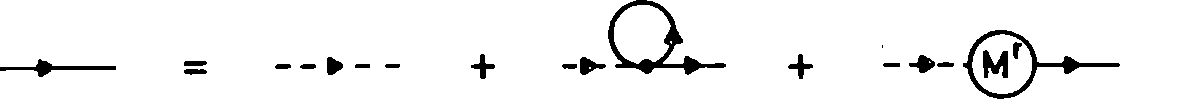
\includegraphics[width=0.7\linewidth]{pictures/Feq38.png}}}\label{eq:F_38}
\end{equation}
其中
\begin{equation}
\vcenter{\hbox{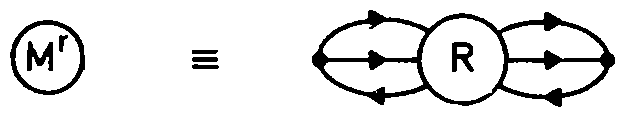
\includegraphics[width=0.4\linewidth]{pictures/Feq39.png}}}\label{eq:F_39}
\end{equation}
这里 $R$ 代表式 \ref{eq:F_25} 和式 \ref{eq:F_21} 中出现的Green函数的特殊组合。式 \ref{eq:F_38}
中的虚线代表式 \ref{eq:F_34} 的完全自由Green函数 $G^{00}$。

为了解析地推导微扰论（其优点在于特定项的系数因子与正负符号可以直接严密得出），我们从所谓的多时间 $n$ 体Green函数的定义出发：
\begin{align}
 & G(1,2,\dots,n;1',2',\dots,n')\nonumber \\
 & =(-\mathrm{i})^{n}\langle0|\mathcal{T}\{a(1)a(2)\dots a(n)a^{\dagger}(n')\dots a^{\dagger}(2')a^{\dagger}(1')\}|0\rangle\nonumber \\
 & =(-\mathrm{i})^{n}\sum_{\text{all permu-}}(-)^{P}\Big\{\Theta(t_{1}-t_{2})\Theta(t_{2}-t_{3})\dots\Theta(t_{n-1}-t_{n})\Theta(t_{n}-t_{n'})\Theta(t_{n'}-t_{(n-1)'})\dots\Theta(t_{2'}-t_{1'})\nonumber \\
 & \quad\cdot\langle0|a(1)a(2)\dots a(n)a^{\dagger}(n')\dots a^{\dagger}(1')|0\rangle\Big\}.\label{eq:F_40}
\end{align}
定义 \ref{eq:F_40} 意味着算符始终按照其时间参数从右到左递增的方式进行编时排列。也很容易看出，表达式 \ref{eq:F_40}
关于任意两个指标的对换是完全反对称的。我们想要写出Green函数 \ref{eq:F_40} 的运动方程，这对于单体和两体情形很容易证明；然而对于一般情况，证明过程相当繁琐，我们建议感兴趣的读者参考标准文献
\cite{Mi67,AGD65}：
\begin{align}
 & G^{00-1}(1,1'')\cdot G(1'',2\dots n;1'\dots n')\nonumber \\
 & =\sum^{n}_{l=1}(-)^{l+1}\delta(1,l')\cdot G(2\dots n;1'\dots l'-1,l'+1,\dots n')\nonumber \\
 & \quad-\frac{\mathrm{i}}{2}\bar{v}(1,n'+1;1'',n+1)\cdot G(1'',2\dots n,(n+1)^{+};1'\dots n',(n'+1)^{++}).\label{eq:F_41}
\end{align}
参数上的正号表示相应的时间参数移位了一个正的无穷小量，即 $1^{+}=p_{1},t_{1}+0$ 以及 $1^{++}=p_{1},t_{1}+0+0$。两体相互作用矩阵元由下式给出：
\begin{equation}
\bar{v}(1,2;3,4)=\delta(t_{1}-t_{2})\delta(t_{3}-t_{4})\delta(t_{1}-t_{3})\bar{v}_{1234}.\label{eq:F_42}
\end{equation}

求逆运动方程 \ref{eq:F_41} 是非常有用的：
\begin{align}
 & G(1\dots n;1'\dots n')\nonumber \\
 & =\sum^{n}_{l=1}(-)^{l+1}G^{00}(1,l')G(2\dots n;1'\dots l'-1,l'+1\dots n')\nonumber \\
 & \quad-\frac{\mathrm{i}}{2}G^{00}(1,1''')\bar{v}(1''',n'+1;1'',n+1)\cdot G(1'',2\dots n,(n+1)^{+};1'\dots n',(n'+1)^{++}).\label{eq:F_43a}
\end{align}
其伴随方程的形式为：
\begin{align}
 & G(1\dots n;1'\dots n')\nonumber \\
 & =\sum^{n}_{l=1}(-)^{l+1}G(1\dots l-1,l+1\dots n;2'\dots n')G^{00}(l,1')\nonumber \\
 & \quad-\frac{\mathrm{i}}{2}G(1\dots n,(n+1)^{++};1'',2'\dots n',(n'+1)^{+})\bar{v}(n'+1,1'';n+1,1''')G^{00}(1''',1').\label{eq:F_43b}
\end{align}
我们看到，运动方程将 $n$ 体Green函数与 $(n\pm1)$ 体Green函数联系了起来。从式 \ref{eq:F_43a}
中，我们很容易推导出完全忽略两体相互作用的近似下 $n$ 体Green函数的表达式 $G^{00}(1\dots n;1'\dots n')$：
\begin{equation}
G^{00}(1\dots n;1'\dots n')=\det|G^{00}(i,j)|.\label{eq:F_44}
\end{equation}

由此，如何计算 $n$ 体Green函数的一阶表达式就十分清楚了：我们首先利用两体Green函数的式 \ref{eq:F_44}
计算单体Green函数的一阶贡献。两体Green函数耦合到单体和三体Green函数。单体Green函数的一阶由前一步已知，而三体Green函数可通过式
\ref{eq:F_44} 计算到零阶；这便得出了两体Green函数的一阶贡献。我们可以按此方案继续推演，以计算 $n$ 体Green函数的一阶。为了计算二阶，我们需要一阶表达式，由此建立起类似的递推方案。这一过程随后可以重复进行到任意阶。

\section{骨架展开}

对于许多问题，我们并不太关心用 $G^{00}(1,1')$ 表示的展开项，而是希望得到按精确 $G(1,1')$ 的幂次展开（骨架展开，skeleton
expansion）。微扰级数的这种部分重求和之所以可能，可以通过仅涉及 $G^{00}(1,1')$ 的级数研究来证明。我们可以通过将式
\ref{eq:F_43a} 从左侧乘以式 \ref{eq:F_19b} 并利用式 (F.9, 12) 来推导骨架展开：
\begin{align}
 & G(1\dots n;1'\dots n')\nonumber \\
 & =\sum^{n}_{l=1}(-)^{l+1}G(1,l')\cdot G(2\dots n;1'\dots l'-1,l'+1\dots n')\nonumber \\
 & \quad-\frac{\mathrm{i}}{2}G(1,1''')\bar{v}(1''',n'+1;1'',n+1)\cdot R(1'',2\dots n,(n+1)^{+};1'\dots n',(n'+1)^{++}),\label{eq:F_45}
\end{align}
其中
\begin{align}
 & R(1\dots n,n+1;1'\dots n',n'+1)\nonumber \\
 & =G(1\dots n,n+1;1'\dots n',n'+1)-G(1,n+1;1'',n'+1)G^{-1}(1'',2'')G(2'',2\dots n;1'\dots n').\label{eq:F_46}
\end{align}
与按 $G^{00}(1,1')$ 幂次展开的情形一样，我们从式 \ref{eq:F_45} 中看出，对于骨架展开，零阶骨架贡献由下式给出：
\begin{equation}
G^{\text{skeleton}}(1\dots n;1'\dots n')\equiv G^{0}(1\dots n;1'\dots n')=\det|G(i,j)|,\label{eq:F_47}
\end{equation}
也就是说，在最低阶骨架近似下，$n$ 体Green函数就是相应单体Green函数的反对称化积。现在基本上按完全自由情形相同的方式推进，我们从式
(F.45, 46, 47) 即可获得骨架展开的连续各阶项。应当注意，式 \ref{eq:F_46} 的最低阶已不再是反对称化积，式
\ref{eq:F_46} 右侧的第二项恰好从第一项中扣除了在式 \ref{eq:F_45} 右侧第一项最低阶中已经重求和过的部分。读者不妨选取一个具体示例亲自验证这一事实。

上述推导骨架展开的规程是清晰明了的，它能自动给出给定阶项的正确符号和前置因子。视具体示例和展开阶数而定，其推导可能相当冗长。为了经济高效地进行这些计算，实际演算练习是必不可少的，这也是所有微扰展开技术的共同特征。为了更熟悉这些步骤，我们建议读者验证以下事实：质量算符动态部分的表达式
\ref{eq:F_25} 包含一个广义三体Green函数 \cite{ES69}：
\begin{equation}
R(1,2,3;1',2',3')=G(1,2,3;1',2',3')-G(1,2;1'',2')G^{-1}(1'',1''')G(1''',3;1',3').\label{eq:F_48}
\end{equation}
验证式 \ref{eq:F_48} 右侧的第一项和第二项（在二阶上）都包含具有图 \ref{fig:F_1} 所示结构的项，且它们恰好相互抵消。人们通常称质量算符的动态部分是单线不可约的（one-line
irreducible），即它不包含仅通过切断一条费米子线就能被分割成两部分的图。进一步的考察表明，式 \ref{eq:F_48}
第二项的所有图都是单线可约的，且这些项精确抵消了式 \ref{eq:F_48} 第一项中所包含的相等项。余下的部分则是不可约的。

\begin{figure}[H]
\begin{centering}
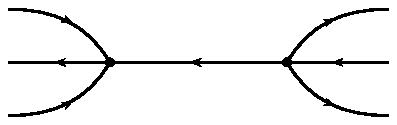
\includegraphics[width=0.4\linewidth]{pictures/F_1}
\par\end{centering}
\caption{\label{fig:F_1}式 (F.48) 中两项的二阶贡献。}
\end{figure}

质量算符的二阶骨架展开可以很容易地从式 \ref{eq:F_48} 结合式 \ref{eq:F_47} 计算得出：
\begin{equation}
M^{(2)}(1,1')=\frac{1}{2}\bar{v}(1,2';1''',2)G(1''',1'')G(2,3')G(3,2')\bar{v}(3',1'';3,1'),\label{eq:F_49}
\end{equation}
其图形表示示于图 \ref{fig:F_2}。在图 \ref{fig:F_3} 中，我们非常示意性地给出了式 \ref{eq:F_48}
中所包含的一些更高阶项。在示意绘图中，我们没有画出交换图。

\begin{figure}[H]
\begin{centering}
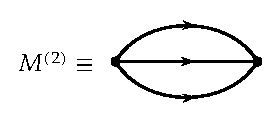
\includegraphics[width=0.35\textwidth]{pictures/F_2}
\par\end{centering}
\caption{\label{fig:F_2}质量算符二阶骨架贡献的图形表示。}
\end{figure}

\begin{figure}[H]
\begin{centering}
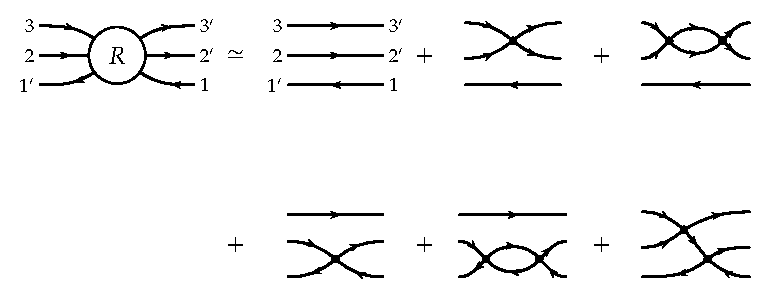
\includegraphics[width=0.75\textwidth]{pictures/F_3}
\par\end{centering}
\caption{\label{fig:F_3}质量算符中所含Green函数的更高阶贡献项。}
\end{figure}


\section{因子化与Brueckner-Hartree-Fock理论}

$n$ 体Green函数的一个重要特征在于它们能够近似因子化为更低阶Green函数的反对称化积。这一点可以通过对相应微扰级数的广泛研究来加以验证。例如在图
\ref{fig:F_3} 中我们看到，前五个图项恰好是如下因子化展开的开端：
\begin{align}
R(1,2,3;1',2',3') & \simeq G(1,1')\cdot G(2,3;2',3')\nonumber \\
 & \quad+\Big\{\left[G(2,2')\cdot R(1,3;1',3')-(3\leftrightarrow2)\right]-\left[3'\leftrightarrow2'\right]\Big\}\nonumber \\
 & \quad+\Big\{\left[G(2,2')\cdot G(1,1')\cdot G(3,3')-(3\leftrightarrow2)\right]-\left[3'\leftrightarrow2'\right]\Big\},\label{eq:F_50}
\end{align}
其中
\begin{equation}
R(1,3;1',3')=G(1,3;1',3')+G(1,3')\cdot G(3,1').\label{eq:F_51}
\end{equation}
函数 \ref{eq:F_51} 本质上等价于式 (8.130) 中定义的线性响应函数\footnote{式 (8.130) 中定义的响应函数在时间坐标空间中对 $t_{1}=t_{1'}$ 和 $t_{3}=t_{3'}$ 由 $-\mathrm{i}\Theta(t_{1}-t_{3})\langle0|[a^{\dagger}(1')a(1),a^{\dagger}(3')a(3)]|0\rangle$
给出。该定义与式 (F.51) 的区别在于式 (8.130) 第二项中 $\mathrm{i}\eta$ 的符号、一个额外的因子
$(-\mathrm{i})$ 以及费米子算符的排列顺序。由于两种定义的物理内容完全相同，我们可以在两种形式下自由切换工作。}；通过将式 \ref{eq:F_51} 与式 (8.131) 进行比对，可以证实我们必须加上式 \ref{eq:F_51} 中的第二项。

初学者容易感到困惑的一个特点是：因子化式 \ref{eq:F_50}——即除单粒子Green函数的三重积之外的所有项——并没有给出式
\ref{eq:F_48} 的正确最低阶骨架项，亦即它未能直接重现表达式 \ref{eq:F_49}。因子化仅对关联部分有效，亦即对式
\ref{eq:F_48} 中所包含的二阶、三阶、四阶、五阶以及所有相应的更高阶图（图 \ref{fig:F_3}）有效。为了修正并配平出正确的最低阶贡献，我们在式
\ref{eq:F_50} 的因子化中必须补加上 $G(i,j)$ 的三重积。另一方面，关联部分求和了式 \ref{eq:F_50}
中出现的精确两体关联函数中所包含的无穷子级数，因此因子化可以构成一种非常强大的近似方案。

我们注意到，式 \ref{eq:F_50} 右侧的第一项求和了粒子-粒子（pp）关联（见图 \ref{fig:F_3}），正如我们在4.3节中所讨论的，这些关联对于处理由裸核子-核子力硬芯所引入的短程关联至关重要。因此，若我们只想处理这些关联，便可以舍去式
\ref{eq:F_50} 中的其他项，并将质量算符写为：
\begin{equation}
M(1,1')=T(1,2;1',4)G(4,2)\label{eq:F_52}
\end{equation}
其中 $T$ 矩阵由下式给出：
\begin{equation}
T(1,2;1',4)=\bar{v}(1,2;1',4)+\frac{1}{4}\bar{v}(1,2;3',4')G(3',4';5,6)\bar{v}(5,6;1',4).\label{eq:F_53}
\end{equation}
对于式 \ref{eq:F_53} 中出现的两体Green函数，存在一个著名的积分方程（见下文）\cite{Mi67}：
\begin{equation}
G(1,2;1',2')=G^{0}(1,2;1',2')-\frac{1}{4}G^{0}(1,2;3,4)K^{pp}(3,4;3',4')G(3',4';1',2'),\label{eq:F_54}
\end{equation}
其中 $K^{pp}$ 是一种有效 pp 力，在最低阶下由下式给出：
\begin{equation}
K^{pp}(3,4;3',4')\simeq\bar{v}(3,4;3',4').\label{eq:F_55}
\end{equation}

如果我们进而利用式 (F.28, 29) 将式 \ref{eq:F_54} 中的单粒子Green函数替换为其HF表达式，并在式 (F.28,
29) 中略去第二部分（空穴贡献；可以证明空穴线在密度展开中属于更高阶，因此被认为显著小于粒子贡献；参见例如 \cite{Ma67b}），结合式
(F.52-55)，我们便求得了Brueckner-Hartree-Fock方程 (5.72) 的结构。我们现在必须认识到，$T$
矩阵 \ref{eq:F_53} 实际上仅依赖于一个时间差，在Fourier变换后引起能量依赖性。如果这一能量依赖性按照式 (5.75)
的规则加以替换，我们就可以将式 \ref{eq:F_52} 和式 \ref{eq:F_53} 与Brueckner-HF方程 (5.72)
严格完全等同起来。

\section{Hartree-Fock-Bogoliubov方程}

不仅推导Brueckner-Hartree-Fock理论非常有益，利用Green函数技术推导Hartree-Fock-Bogoliubov（HFB）理论同样富有启发性。为此，我们再次仅保留式
\ref{eq:F_50} 右侧的第一项，因为我们已经知道配对关联属于 pp 关联。式 \ref{eq:F_50} 第一项中的空穴Green函数
$G(1,1')$ 是仅使用质量算符的静态部分计算的。对于两体Green函数，我们需要给出其谱表示：
\begin{align}
G_{12,1'2'}(t-t') & =(-\mathrm{i})^{2}\langle0|\mathcal{T}\{a_{1}(t)a_{2}(t)a^{\dagger}_{2'}(t')a^{\dagger}_{1'}(t')\}|0\rangle\nonumber \\
 & =(-\mathrm{i})^{2}\Big\{\Theta(t-t')\sum_{\rho^{+}}\langle0|a_{1}a_{2}|\rho^{+}\rangle\langle\rho^{+}|a^{\dagger}_{2'}a^{\dagger}_{1'}|0\rangle\mathrm{e}^{-(\mathrm{i}/\hbar)(E^{A+2}_{\rho}-E^{A}_{0})(t-t')}\nonumber \\
 & \quad+\Theta(t'-t)\sum_{\rho^{-}}\langle0|a^{\dagger}_{2'}a^{\dagger}_{1'}|\rho^{-}\rangle\langle\rho^{-}|a_{1}a_{2}|0\rangle\mathrm{e}^{-(\mathrm{i}/\hbar)(E^{A}_{0}-E^{A-2}_{\rho})(t-t')}\Big\}\label{eq:F_56}
\end{align}
或者在Fourier变换之后：
\begin{equation}
G_{12,1'2'}(\omega)=(-\mathrm{i})\left\{ \sum_{\rho^{+}}\frac{\langle0|a_{1}a_{2}|\rho^{+}\rangle\langle\rho^{+}|a^{\dagger}_{2'}a^{\dagger}_{1'}|0\rangle}{\omega-\Omega^{pp}_{\rho}+\mathrm{i}\eta}-\sum_{\rho^{-}}\frac{\langle0|a^{\dagger}_{2'}a^{\dagger}_{1'}|\rho^{-}\rangle\langle\rho^{-}|a_{1}a_{2}|0\rangle}{\omega-\Omega^{hh}_{\rho}-\mathrm{i}\eta}\right\} ,\label{eq:F_57}
\end{equation}
其中 $E^{A\pm2}_{\rho},E^{A}_{0}$ 是精确本征能量，且
\[
\hbar\Omega^{pp}_{\rho}=E^{A+2}_{\rho}-E^{A}_{0},\quad\hbar\Omega^{hh}_{\rho}=E^{A}_{0}-E^{A-2}_{\rho}.
\]

HFB理论隐含地假定在式 \ref{eq:F_57} 的 $\rho$ 求和中只有基态是起主导作用的，也就是说，它们被假定具有高度的集体性，以至于在式
\ref{eq:F_57} 的留数求和（它是一个常数）中，基态的留数汇集了几乎全部的强度。正如我们在第11章中所阐述的，特定模式的集体性概念是相变（在此即向超流态的相变）的核心本质特征。

牢记式 \ref{eq:F_50} 第一项中的单粒子Green函数在质量算符中演化为空穴线，利用式 (F.21)、式 (F.22)
和式 \ref{eq:F_50}，我们在质量算符的动态部分中分离出所谓的Cooper极点 \cite{Pi61}\footnote{我们应当注意到，对于空穴线，Dyson方程的方向是反转的，因此在式 (F.58) 中出现的是单粒子势的复共轭。这也可以在微扰论中针对式
(F.39) 中的 $R$ 函数加以验证。然而，这一点仅在单粒子Hamilton量不具备时间反演不变性时才具有实际意义。}，从而获得如下近似Dyson方程 {[}推导时应完全在时间坐标空间中利用式 (F.29) 进行，仅在最后一步执行Fourier变换{]}：
\begin{align}
(\hbar\omega-\varepsilon_{1})G_{11'}(\omega) & =\delta_{11'}+\bar{v}_{1234}\rho_{42}G_{31'}(\omega)+M^{\text{Cooper}}_{12}\cdot G_{21'}(\omega),\nonumber \\
M^{\text{Cooper}}_{11'}(\omega) & =\Delta^{(+)}_{12}\cdot\left(\frac{\rho}{\hbar\omega-\hbar\Omega^{pp}_{0}+h^{*}}\right)_{22'}\cdot\Delta^{(+)*}_{2'1'}\nonumber \\
 & \quad+\Delta^{(-)}_{12}\cdot\left(\frac{1-\rho}{\hbar\omega-\hbar\Omega^{hh}_{0}+h^{*}}\right)_{22'}\cdot\Delta^{(-)*}_{2'1'},\label{eq:F_58}
\end{align}
其中
\begin{align}
\Delta^{(+)}_{12} & =-\frac{1}{2}\bar{v}_{1234}\langle0|a_{3}a_{4}|A+2,0\rangle,\nonumber \\
\Delta^{(-)}_{12} & =-\frac{1}{2}\bar{v}_{1234}\langle A-2,0|a_{3}a_{4}|0\rangle.\label{eq:F_59}
\end{align}
因为我们只考虑束缚态问题，所以可以忽略式 \ref{eq:F_58} 分母中的无穷小量 $\pm\mathrm{i}\eta$。针对向超流态相变的情况，我们可以作出的下一个近似是：
\begin{align}
\hbar\Omega^{pp}_{0} & \simeq2(E^{A+1}_{0}-E^{A}_{0})=2\lambda^{(+)},\nonumber \\
\hbar\Omega^{hh}_{0} & \simeq2(E^{A}_{0}-E^{A-1}_{0})=2\lambda^{(-)}.\label{eq:F_60}
\end{align}
这一近似意味着构成Cooper对的两个粒子的关联能为零。这当然是我们在处理相变时可以作出的另一个假设：特定激发模变得如此之软，以致其激发能趋近于零。最后，我们假定对于大系统可以进一步作出粒子数不守恒近似（该近似也可以避免
\cite[1.4.6节]{Mi67}）：
\begin{equation}
\Delta^{(+)}\simeq\Delta^{(-)}=\Delta;\quad\lambda^{(+)}\simeq\lambda^{(-)}=\lambda.\label{eq:F_61}
\end{equation}
由此我们便导出了著名的Gorkov方程 \cite{Go58}：
\begin{align*}
(\hbar\omega'-h')_{12}G_{21'} & =\hbar\delta_{11'}-\Delta_{12}F^{*}_{21'},\\
(\hbar\omega'+h'^{*})_{12}F^{*}_{21'} & =\Delta^{*}_{12}G_{21'},
\end{align*}
或写成矩阵形式：
\begin{equation}
\begin{pmatrix}\hbar\omega' & 0\\
0 & \hbar\omega'
\end{pmatrix}_{12}\begin{pmatrix}G\\
-F^{*}
\end{pmatrix}_{21'}=\begin{pmatrix}\hbar\delta_{11'}\\
0
\end{pmatrix}+\begin{pmatrix}h' & \Delta\\
-\Delta^{*} & -h'^{*}
\end{pmatrix}_{12}\begin{pmatrix}G\\
-F^{*}
\end{pmatrix}_{21'},\label{eq:F_62}
\end{equation}
其中我们引入了记号 $\hbar\omega'=\hbar\omega-\lambda,h'=h-\lambda$，且
\begin{equation}
F^{*}_{11'}=-\left(\frac{1}{\hbar\omega'+h'^{*}}\right)_{12}\Delta^{*}_{22'}G_{2'1'}.\label{eq:F_63}
\end{equation}

在式 \ref{eq:F_62} 的右侧，我们认出了式 (7.39) 中熟悉的HFB矩阵 $\mathcal{H}$。照例，我们可以写出
$G(1,1')$ 的谱表示 (F.6a, b)，并且从式 \ref{eq:F_63} 中看出对于 $F^{*}(1,1')$
同样可以建立谱表示：
\begin{align}
G_{11'}(\omega) & =\hbar\sum_{k}\frac{V^{*}_{1k}V_{1'k}}{\hbar\omega+E_{k}-\mathrm{i}\eta}+\frac{U_{1k}U^{*}_{1'k}}{\hbar\omega-E_{k}+\mathrm{i}\eta},\nonumber \\
-F^{*}_{11'}(\omega) & =\hbar\sum_{k}\frac{U^{*}_{1k}V_{1'k}}{\hbar\omega+E_{k}-\mathrm{i}\eta}+\frac{V_{1k}U^{*}_{1'k}}{\hbar\omega-E_{k}+\mathrm{i}\eta}.\label{eq:F_64}
\end{align}
从式 \ref{eq:F_64} 中我们发现，在极点处方程 \ref{eq:F_62} 与HFB方程 (7.42) 完全等同。

为了闭合该方程组，我们必须阐明如何从解 $G_{11'},F^{*}_{11'}$ 中求得配对能隙 $\Delta$。为此，我们将式
\ref{eq:F_59} 中出现的跃迁振幅表述为：
\begin{equation}
\langle0|a_{3}a_{4}|A+2,0\rangle=\lim_{\substack{t=t_{2}=t_{1}+0\rightarrow-\infty\\
t_{3}=t_{4}+0\rightarrow0
}
}\exp(-\mathrm{i}\Omega^{pp}_{0}t)\frac{\langle0|\mathcal{T}\{a(3)a(4)a^{\dagger}(2)a^{\dagger}(1)\}|0\rangle}{\langle A+2,0|a^{\dagger}_{2}a^{\dagger}_{1}|0\rangle}.\label{eq:F_65}
\end{equation}
该关系式 \cite{WE70} 可以通过从时间极限过渡到Abel极限来证明其成立：
\begin{align}
|A+2,0\rangle & =\lim_{\eta\rightarrow0}\eta\int^{0}_{-\infty}\mathrm{d}t\,\mathrm{e}^{\eta t}\frac{\mathrm{e}^{-\mathrm{i}\Omega^{pp}_{0}t}}{\langle A+2,0|a^{\dagger}_{2}a^{\dagger}_{1}|0\rangle}a^{\dagger}_{2}(t)a^{\dagger}_{1}(t)|0\rangle\nonumber \\
 & =\lim_{\eta\rightarrow0}\frac{\eta}{\langle A+2,0|a^{\dagger}_{2}a^{\dagger}_{1}|0\rangle}\sum_{\tau}\frac{\langle A+2,\tau|a^{\dagger}_{2}a^{\dagger}_{1}|0\rangle}{-\mathrm{i}(E^{A+2}_{0}-E^{A+2}_{\tau}+\mathrm{i}\eta)}|A+2,\tau\rangle\nonumber \\
 & =|A+2,0\rangle.\quad\text{证毕（Q.E.D.）}\label{eq:F_66}
\end{align}
对于式 \ref{eq:F_65} 中出现的两体Green函数，我们可以利用积分方程 \ref{eq:F_54}；将 $K^{pp}$
前面的单粒子Green函数之一替换为其最低阶表达式 \ref{eq:F_26}，并将具有式 \ref{eq:F_55} 的式 \ref{eq:F_54}
代入式 \ref{eq:F_65} 中，结合式 \ref{eq:F_61} 和式 \ref{eq:F_63}，我们便得到了“能隙方程”：
\begin{equation}
\Delta_{12}=\frac{1}{2}\bar{v}_{1234}\frac{1}{2\pi\mathrm{i}}\oint\mathrm{d}\omega\,F_{34}(\omega).\label{eq:F_67}
\end{equation}
因此，结合式 \ref{eq:F_62}，我们获得了完全闭合的自洽方程组。我们在式 \ref{eq:F_54} 中将其中一个单粒子Green函数替换为其最低阶表达式
\ref{eq:F_26}，表面上看起来似乎是对式 \ref{eq:F_54} 中两个单粒子Green函数的非对称处理；然而，正如Gorkov方程
\ref{eq:F_62} 的推导所表明的，这与质量算符的近似 \ref{eq:F_58} 是完全内在自洽的。

我们想对刚刚推导出的这组耦合方程给出图形化与物理学解释。方程 \ref{eq:F_58} 在图 \ref{fig:F_4}a 中给出图形表示，而方程
\ref{eq:F_67} 则在图 \ref{fig:F_4}b 中表示。

\begin{figure}[H]
\begin{centering}
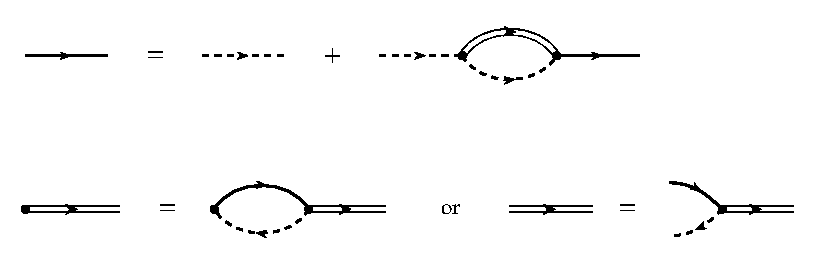
\includegraphics[width=0.7\textwidth]{pictures/F_4}
\par\end{centering}
\caption{\label{fig:F_4}(a) 式 (F.58) 的图形表示，其中虚线代表最低阶近似 (F.26)，双线代表配对模。(b)
能隙方程 (F.67) 的图形表示。}
\end{figure}

从图 \ref{fig:F_4} 中我们可以看出，用Green函数的语言来表达，HFB方程的物理内涵在于：配对模是由单粒子传播子计算得出的，而这些传播子本身又通过粒子与配对模及空穴的耦合而发生重整化。这些耦合方程的求解隐含地求和了微扰级数的一个重要组成部分，从而允许我们描述宏观相变。

在推导Brueckner-HF理论和HFB理论时，我们最初对质量算符采用了相同的近似形式 {[}式 \ref{eq:F_50} 右侧的第一项{]}，这可能会让人感到困惑。然而应当认识到，Brueckner-HF理论从未分离出式
\ref{eq:F_50} 两体Green函数中所包含的Cooper极点。我们在HFB理论中显式地处理这一极点，因此与Brueckner-HF并不冲突；我们也可以在统一的Brueckner-HFB理论框架下将这两种理论结合起来。

到目前为止，我们讨论了从正常态到超流态的相变，并展示了某一个特定的 pp 模如何汇集几乎全部集体性，并随之变得非常软，从而使我们能够导出HFB方程。从我们早先的考察（参见第7章）可知，HFB方程允许球形解（保持空间转动对称性）和形变解（破缺空间转动对称性）。然而在我们对配对现象的处理中，我们未曾在任何地方假设过转动对称性的破缺——我们始终假定
$\rho_{11'}=\langle0|a^{\dagger}_{1'}a_{1}|0\rangle$ 对应于具有良好角动量的基态密度（为了明确思路，例如对偶偶核取
$I=0$）。从第7章和第11章关于从球形核向形变核相变的论述中，我们知道这恰好与另一种软模——四极振动相关联。我们将更详细地展示这在Green函数形式体系中是如何描述的。

显而易见，为了处理从球形态向形变态的转变，我们必须在质量算符 \ref{eq:F_25} 中分离出粒子与四极声子的耦合。这可以通过仅从因子化式
\ref{eq:F_50} 中保留出现响应函数 \ref{eq:F_51} 的那些项来最容易地实现。谱分解随后给出了 $A$
体系统的激发能 (8.130)：
\begin{equation}
R_{13,1'3'}(\omega)=\mathrm{i}\sum_{\mu>0}\left(\frac{\langle0|a^{\dagger}_{1'}a_{3'}|\mu\rangle\langle\mu|a^{\dagger}_{3}a_{1}|0\rangle}{\omega-\Omega^{ph}_{\mu}+\mathrm{i}\eta}-\frac{\langle0|a^{\dagger}_{3}a_{1}|\mu\rangle\langle\mu|a^{\dagger}_{1'}a_{3'}|0\rangle}{\omega+\Omega^{ph}_{\mu}-\mathrm{i}\eta}\right).\label{eq:F_68}
\end{equation}
如同处理配对模的情形一样，我们现在假定式 \ref{eq:F_68} 中最低的激发几乎耗尽了全部的跃迁强度，并且其激发能趋近于零（$\Omega^{ph}_{\mu}\rightarrow0$）。在此我们假定四极模通常具有这种性质（确实，对于转动核，其激发能变得非常低）；然而，有时其他激发模也可能成为最低的激发态（例如在
$^{208}\text{Pb}$ 中）。对于式 \ref{eq:F_50} 中出现的单粒子Green函数，我们再次采用最低阶近似
\ref{eq:F_26}。Dyson方程于是具有如下形式：
\begin{align}
(\hbar\omega-\varepsilon_{1})G_{11'}(\omega) & =\delta_{11'}+\bar{v}_{1234}\rho_{42}G_{31'}(\omega)+M^{\text{phonon}}_{12}G_{21'}(\omega),\label{eq:F_69}
\end{align}
其中
\begin{equation}
M^{\text{phonon}}_{11'}(\omega)=Q^{\overbracket{2^{+}2}}_{1}\left(\frac{1}{\hbar\omega-h}\right)_{22'}Q^{\overbracket{2^{+}2'}*}_{1'},\label{eq:F_70}
\end{equation}
以及
\begin{equation}
Q^{\overbracket{2^{+}2}}_{1}=\bar{v}_{1(324)_{j_{1}}}\langle0|[a^{\dagger}_{3}a_{4}]_{2^{+}}|2^{+}\rangle.\label{eq:F_71}
\end{equation}

应当指出，到目前为止我们尚未作出任何破缺对称性的近似，因为——正如符号所指明的——所有量都已耦合到良好角动量（我们将粒子 2 或 $2'$
与四极声子耦合以给出外场粒子的角动量 $j_{1}$）。我们还应当认识到，式 \ref{eq:F_71} 中的 $Q$ 场对应于9.3.3节中粒子-振动耦合理论的
$\gamma$ 顶点（不含因子 $\frac{1}{2}$；见第386页脚注讨论）。通过引入如下量：
\begin{equation}
P_{11'}=-\left(\frac{1}{\hbar\omega-h}\right)_{12}Q^{\overbracket{2^{+}2}*}_{2'}G_{2'1'},\label{eq:F_72}
\end{equation}
我们可以再次将式 (F.69, 70) 改写为两个相互耦合的方程形式：
\begin{align}
(\hbar\omega-h)_{12}G_{21'}(\omega) & =\delta_{11'}+Q^{\overbracket{2^{+}2}}_{1}P^{*}_{21'}(\omega),\nonumber \\
(\hbar\omega-h)_{12}P^{*}_{21'}(\omega) & =-Q^{\overbracket{2^{+}1}*}_{2}G_{21'}(\omega).\label{eq:F_73}
\end{align}
如同配对的情形一样，我们必须使方程组闭合。在此可以通过使用响应函数的Bethe-Salpeter方程 (8.131) 来代替式 \ref{eq:F_50}，从而以完全类似的方式达成这一目标。其结果为：
\begin{equation}
\langle0|[a^{\dagger}_{3}a_{4}]_{2^{+}}|2^{+}\rangle=\delta\rho^{(2^{+})}_{43}=\frac{1}{2\pi\mathrm{i}}\oint\mathrm{d}\omega\,P_{43}(\omega).\label{eq:F_74}
\end{equation}
将式 \ref{eq:F_74} 代入式 \ref{eq:F_71} 中，连同式 \ref{eq:F_73} 一起，便构成了形变场“序参量”
$Q$ 的“能隙方程”。

两个单粒子场进入方程组 (F.73)，一个涉及普通密度 $\rho_{12}=\langle0|a^{\dagger}_{2}a_{1}|0\rangle$，另一个涉及跃迁密度
\[
\delta\rho^{(2^{+})}_{12}=\langle0|[a^{\dagger}_{2}a_{1}]_{2^{+}}|2^{+}\rangle.
\]
跃迁密度自然投影出了式 \ref{eq:F_71} 中 $ph$ 力的四极部分，而普通密度则投影出了式 \ref{eq:F_69}
中力的单极部分。我们再次强调：到目前为止没有作出任何破坏对称性的近似，因为我们已经把所有量都耦合到了良好的角动量。形变HF理论的对称性破缺可以通过将
$2^{+}$ 态等同于内禀系统的基态而引入。在此时，进行角动量耦合便不再有意义，方程 \ref{eq:F_73} 随即退化为通常的形变HF方程。我们显式地求出了在11.2节中引入的两个势
$V_{0}$ 与 $\Gamma_{2}$，它们现在构成了内禀系统的非角动量守恒单粒子Hamilton量。

正如我们已经指出的，形变场的“能隙方程” (F.71, 74) 同样可以从响应函数的Bethe-Salpeter方程 (8.131)
导出。然而从式 \ref{eq:F_74} 和式 \ref{eq:F_72} 可以看出，它可以图形化地表示为图 \ref{fig:F_5}b
所示的形式。方程 \ref{eq:F_69} 则表示在图 \ref{fig:F_5}a 中。图 \ref{fig:F_5}a,
b 再次清晰地揭示了单粒子运动与集体振动的典型非线性耦合。

\begin{figure}[H]
\begin{centering}
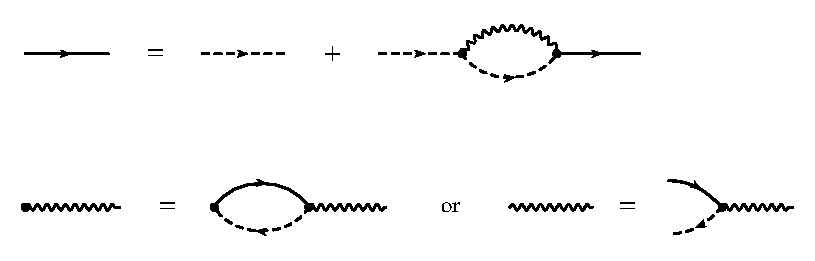
\includegraphics[width=0.7\textwidth]{pictures/F_5}
\par\end{centering}
\caption{\label{fig:F_5}(a) 方程 (F.69) 的图形表示，波浪线代表软四极声子。(b) 形变场 \$Q\$ 的“能隙方程”图形表示。}
\end{figure}

一般而言，我们当然应当在质量算符中同时分离出Cooper极点以及所有多极性的声子极点，从而生成我们在第7章中讨论的一般单粒子理论。从式
\ref{eq:F_71} 和式 \ref{eq:F_59} 中我们看到，跃迁密度进入了形变场和配对场。由于我们已经看到这些密度在核表面处达到峰值（第8章与第13章），因此将进入式
\ref{eq:F_71} 和式 \ref{eq:F_59} 的力替换为可分离力可能是一种极佳的近似。这自然导出了第7章讨论的配对加四极模型，因此我们在核相变的背景下再次领会了该模型的深刻意义。

从该理论的Green函数处理中，也可以清楚地看出一种可能的推广应如何运作：其核心特征在于将RPA模与单粒子态自洽地求解，也就是说，单粒子态以图
\ref{fig:F_5}a, b 所示的方式反作用耦合回到RPA模。此外，HFB理论的对称性守恒表述 \ref{eq:F_62}
应当是该理论的一个极具吸引力的变体；事实上，Janssen 已经提出了这种类型的一种更为精细的理论 \cite{Ja79}。

\section{Bethe-Salpeter方程与有效力}

在推导HFB方程的过程中，我们多次提到了针对两体Green函数的Bethe-Salpeter方程（BSE）。鉴于这些方程在许多教科书中均有详尽推导
\cite{Mi67,AGD65,FW71}，我们在此仅作极其简略的叙述。响应函数 \ref{eq:F_51} 的BSE由下式给出：
\begin{align}
R(1,3;1',3') & =G(1,1')G(3,3')\nonumber \\
 & \quad-G(3,5)G(6,1')K^{ph}(5,7;6,8)R(1,8;7,3').\label{eq:F_75}
\end{align}
方程 \ref{eq:F_75} 是一个精确方程，其中 $K^{ph}$ 被称为有效粒子-空穴力；它对响应函数中仅切断两条线无法被分割为两部分的骨架图进行了全求和。BSE
\ref{eq:F_75} 在图 \ref{fig:F_6} 中给出了图形表示，同时画出了对 $K^{ph}$ 的典型二阶贡献。我们看到，对
$K^{ph}$ 的这些贡献唯有切断四条线才能被分割成两半。方程 \ref{eq:F_75} 可以在骨架微扰展开的任意阶上加以验证。式
\ref{eq:F_75} 中的重复指标照例表示对量子数求和以及对时间积分。值得提及的是，式 \ref{eq:F_75} 在推导形式关系时有时非常方便。然而，超越RPA处理式
\ref{eq:F_75} 是极其复杂的，因为其积分核通常依赖于三个时间（在考虑了时间平移不变性之后）或三个能量。因此在实际应用中，我们有时使用核仅依赖于一个能量的响应函数积分方程
\cite{Sch71c,Sch76}。通过这种方式，我们得出了玻色子（RPA）的Dyson方程，其中包含玻色子质量算符，与费米子的Dyson方程
\ref{eq:F_22b} 非常类似 \cite{SE73,Sch76}。对关联函数的这种处理方式在精神上类似于在凝聚态领域中被称为Mori理论
\cite{Mo65} 的方法。在核物理中，该方法由 Werner 加以应用 \cite{We76,We78}。

\begin{figure}[H]
\begin{centering}
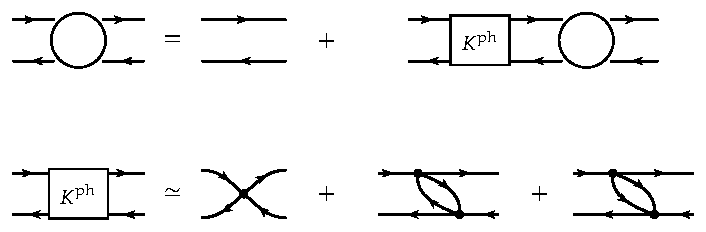
\includegraphics[width=0.7\textwidth]{pictures/F_6}
\par\end{centering}
\caption{\label{fig:F_6}响应函数 (F.50) 的Bethe-Salpeter方程及 \$K\textasciicircum\{ph\}\$
最低阶贡献的示意图。}
\end{figure}

我们关于响应函数的BSE所说的一切，对于两体Green函数的类似BSE \ref{eq:F_54} 同样完全成立：
\begin{align*}
G(1,2;1'2') & =G^{0}(1,2;1',2')-\frac{1}{4}G^{0}(1,2;3,4)K^{pp}(3,4;3',4')G(3',4';1',2').
\end{align*}
在此，$K^{pp}$ 再次求和了所有贡献于 $G(1,2;1',2')$ 且仅切断两条骨架线无法分为两半的图。在图 \ref{fig:F_7}
中，我们给出了式 \ref{eq:F_54} 的图形表示，以及对 $K^{pp}$ 的二阶骨架贡献；其最低阶自然就是裸相互作用本身。

\begin{figure}[H]
\begin{centering}
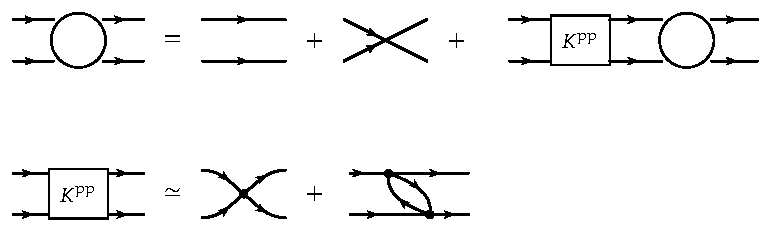
\includegraphics[width=0.75\textwidth]{pictures/F_7}
\par\end{centering}
\caption{\label{fig:F_7}式 (F.54) 的 \$pp\$ Green函数的Bethe-Salpeter方程及 \$K\textasciicircum\{pp\}\$
最低阶贡献的示意图。}
\end{figure}

正如我们在前文中所展示的，配对场 $\Delta$ 的能隙方程 \ref{eq:F_67} 和形变场 $Q$ 的能隙方程 \ref{eq:F_71}
可以分别从相应的Bethe-Salpeter方程 \ref{eq:F_54} 和 \ref{eq:F_75} 导出。因此显而易见，这些序参量必须分别使用相应的有效
$pp$ 力 $K^{pp}$ 和 $ph$ 力 $K^{ph}$ 进行计算。显式地证明这一点是相当精细的，给出全部细节会非常冗长，因此我们在此仅勾勒主要特征。

我们已经证明了在 $\Delta$ 和 $Q$ 的能隙方程中必须分别使用 $K^{pp}$ 和 $K^{ph}$。而要证明
$K^{pp}$ 和 $K^{ph}$ 分别如何在方程 \ref{eq:F_62} 和 \ref{eq:F_73} 的第一个方程中发挥作用则更为复杂。让我们将质量算符
\ref{eq:F_25} 中出现的 $R$ 函数记为 $R_{6}$；则对于质量算符，我们可以采用显而易见的简写记号写出：
\begin{equation}
M'(\omega)=\bar{v}R_{6}R^{-1}_{6}R_{6}\bar{v}.\label{eq:F_76}
\end{equation}
我们已经看到，HFB理论对应于将 $R_{6}$ 近似为式 \ref{eq:F_50} 右侧的第一项，我们将其记为 $GG_{4}$。在这一近似下，我们自然还有：
\begin{equation}
R^{-1}_{6}=[GG_{4}]^{-1}.\label{eq:F_77}
\end{equation}
我们现在注意到，从式 \ref{eq:F_45} 和式 \ref{eq:F_46} 我们有：
\begin{align}
G(1,2;1',2') & =G^{0}(1,2;1',2')\nonumber \\
 & \quad-\frac{\mathrm{i}}{2}R(1,2,3^{++};1'',2',3'^{+})\bar{v}(3',1'';3,1''')\cdot G(1''',1').\label{eq:F_78}
\end{align}
结合式 \ref{eq:F_54}，我们推导出恒等式：
\begin{align}
 & R(1,2,3^{++};1'',2',3'^{+})\bar{v}(3',1'';3,1''')\nonumber \\
 & =G(2,3^{++};2',3'^{+})\cdot G(1,1'')K^{pp}(3',1'';3,1''').\label{eq:F_79}
\end{align}
将式 \ref{eq:F_76} 中的部分 $R_{6}\bar{v}$ 和 $\bar{v}R_{6}$ 分别用式 \ref{eq:F_79}
及其伴随形式替换，并利用式 \ref{eq:F_77}，我们看出在式 \ref{eq:F_58} 和式 \ref{eq:F_62}
中我们必须处处使用 $K^{pp}$。类似地，我们当然也可以证明在式 \ref{eq:F_69} 和式 \ref{eq:F_73}
中必须处处使用 $K^{ph}$。可以证明 \cite{ES69}，我们通过近似 \ref{eq:F_77} 所忽略的项正是图
\ref{fig:F_8} 所示的类型，其中空穴从配对模发生散射。

\begin{figure}[H]
\begin{centering}
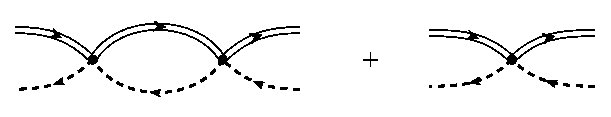
\includegraphics[width=0.5\textwidth]{pictures/F_8}
\par\end{centering}
\caption{\label{fig:F_8}式 (F.77) 近似中所略去的空穴-配对模散射过程。}
\end{figure}

至此我们结束对Green函数理论的简要概述，有关标准技术的更多细节，我们再次建议读者参阅本附录所引用的经典文献。
